\documentclass[aspectratio=169]{beamer}
% SGSSS Beamer Preamble — shared across all lectures
% Brand colours from SGSSS logo

\usetheme{metropolis}

% --- Colour definitions ---
\definecolor{sgsssMagenta}{HTML}{A3217A}
\definecolor{sgsssGreen}{HTML}{2D6A3F}
\definecolor{sgsssBlack}{HTML}{1D1D1B}
\definecolor{sgsssWhite}{HTML}{FFFFFF}
\definecolor{sgsssLightGrey}{HTML}{F5F5F5}

% --- Metropolis colour overrides ---
\setbeamercolor{palette primary}{bg=sgsssMagenta, fg=sgsssWhite}
\setbeamercolor{title separator}{fg=sgsssGreen}
\setbeamercolor{progress bar}{fg=sgsssGreen, bg=sgsssLightGrey}
\setbeamercolor{frametitle}{bg=sgsssMagenta, fg=sgsssWhite}
\setbeamercolor{alerted text}{fg=sgsssMagenta}
\setbeamercolor{example text}{fg=sgsssGreen}
\setbeamercolor{block title}{bg=sgsssMagenta, fg=sgsssWhite}
\setbeamercolor{block body}{bg=sgsssLightGrey, fg=sgsssBlack}
\setbeamercolor{block title example}{bg=sgsssGreen, fg=sgsssWhite}
\setbeamercolor{block body example}{bg=sgsssLightGrey, fg=sgsssBlack}
\setbeamercolor{block title alerted}{bg=sgsssMagenta, fg=sgsssWhite}
\setbeamercolor{block body alerted}{bg=sgsssLightGrey, fg=sgsssBlack}
\setbeamercolor{normal text}{fg=sgsssBlack}

% --- Fonts ---
\usepackage[T1]{fontenc}
\usepackage[sfdefault]{FiraSans}
\usepackage{FiraMono}
\setbeamerfont{frametitle}{size=\large}

% --- Packages ---
\usepackage{graphicx}
\usepackage{bookmark}
\hypersetup{
    bookmarks=true,
    bookmarksopen=true,
    bookmarksdepth=2,
    pdfpagemode=UseOutlines,
}
% --- PDF bookmarks for each frame title ---
\makeatletter
\apptocmd{\beamer@@frametitle}{%
  \only<1>{\bookmark[page=\the\c@page,level=1]{#1}}%
}{}{}
\makeatother
\usepackage{array}
\usepackage{booktabs}
\usepackage{minted}
\usepackage{fontawesome5}

% --- TikZ ---
\usepackage{tikz}
\usetikzlibrary{arrows.meta, positioning, shapes.geometric, trees, calc, decorations.pathmorphing, decorations.pathreplacing, fit, backgrounds}

% Reusable TikZ styles
\tikzset{
    server node/.style={rectangle, draw=sgsssGreen, fill=sgsssGreen!10, thick, minimum width=2.5cm, minimum height=1.2cm, align=center, font=\small},
    client node/.style={rectangle, draw=sgsssMagenta, fill=sgsssMagenta!10, thick, minimum width=2.5cm, minimum height=1.2cm, align=center, font=\small},
    api node/.style={rectangle, draw=sgsssGreen, fill=sgsssGreen!15, thick, rounded corners, minimum width=2.5cm, minimum height=1.2cm, align=center, font=\small},
    data node/.style={rectangle, draw=sgsssBlack, fill=sgsssLightGrey, thick, minimum width=2cm, minimum height=1cm, align=center, font=\small},
    arrow style/.style={-{Stealth[length=3mm]}, thick, sgsssBlack},
    html tag/.style={rectangle, draw=sgsssMagenta, fill=sgsssMagenta!8, rounded corners=2pt, font=\ttfamily\small, inner sep=4pt},
    json key/.style={rectangle, draw=sgsssGreen, fill=sgsssGreen!8, rounded corners=2pt, font=\ttfamily\small, inner sep=4pt},
}

% --- Minted configuration ---
\setminted{
    fontsize=\footnotesize,
    frame=leftline,
    framesep=2mm,
    baselinestretch=1.1,
    bgcolor=sgsssLightGrey,
    breaklines,
    linenos=false,
}
\setminted[python]{style=friendly}
\setminted[r]{style=friendly}

% --- Convenience commands ---
\newcommand{\pythoncode}[1]{\mintinline{python}{#1}}
\newcommand{\rcode}[1]{\mintinline{r}{#1}}
\newcommand{\httpstatus}[2]{\texttt{#1} \textit{#2}}

% --- Footer (page numbers only; logo on title slide only) ---
\setbeamertemplate{frame footer}{%
    \insertframenumber/\inserttotalframenumber%
}

% --- Metadata ---
\author{Dr Diarmuid McDonnell}
\institute{Braw Data Ltd \and Gradel Institute of Charity, University of Oxford}
\date{27 March 2026}


\title{Topic Modelling: Discovering Themes in Text}
\subtitle{SGSSS Training Course}

\begin{document}

% -------------------------------------------------------
% Slide 1: Section title
% -------------------------------------------------------
{
\setbeamertemplate{frame footer}{}
\begin{frame}[plain]
    \begin{center}
        \vspace{1.5cm}
        {\Large\bfseries\color{sgsssMagenta} Topic Modelling}\\[0.3cm]
        {\large Discovering Themes in Text}\\[0.8cm]
        {\normalsize Dr Diarmuid McDonnell}\\[0.1cm]
        {\small Braw Data Ltd \(\cdot\) Gradel Institute of Charity, University of Oxford}\\[0.3cm]
        {\small 27 March 2026}
    \end{center}
\end{frame}
}

% -------------------------------------------------------
% Slide 2: What is topic modelling?
% -------------------------------------------------------
\begin{frame}{What Is Topic Modelling?}
    \begin{alertblock}{Key idea}
        An \textbf{unsupervised} method for discovering \textbf{latent themes} (topics) in a collection of documents --- no labels or pre-defined categories required.
    \end{alertblock}

    \textbf{Analogy:} imagine a reader sorting a large pile of documents into thematic groups \textit{without being told what the themes are}. Topic modelling automates this process.

    \vspace{0.3cm}
    \begin{itemize}\setlength\itemsep{0pt}
        \item \faIcon{layer-group} Documents are \textbf{mixtures} of topics --- a speech can be partly about health, partly about the economy
        \item \faIcon{cogs} The algorithm discovers topics by identifying \textbf{word co-occurrence patterns}
        \item \faIcon{users} Widely used in political science, sociology, media studies, and digital humanities
    \end{itemize}
\end{frame}

% -------------------------------------------------------
% Slide 3: LDA intuition (part 1) — generative model
% -------------------------------------------------------
\begin{frame}{LDA Intuition: The Generative Story}
    \small
    \textbf{Latent Dirichlet Allocation} (Blei, Ng \& Jordan, 2003) imagines each document was ``generated'' by:

    \vspace{0.2cm}
    \begin{center}
    \begin{tikzpicture}[node distance=0.8cm and 1.8cm]
        % Styles (separate styles to avoid parameterised #1 inside beamer frame)
        \tikzset{
            gen step/.style={rectangle, draw=sgsssMagenta, fill=sgsssMagenta!10, thick,
                rounded corners=3pt, minimum width=3cm, minimum height=0.9cm, align=center, font=\small},
            word green/.style={rectangle, draw=sgsssGreen, fill=sgsssGreen!15, thick, rounded corners=2pt,
                minimum width=0.7cm, minimum height=0.5cm, font=\scriptsize\bfseries},
            word magenta/.style={rectangle, draw=sgsssMagenta, fill=sgsssMagenta!15, thick, rounded corners=2pt,
                minimum width=0.7cm, minimum height=0.5cm, font=\scriptsize\bfseries},
        }

        % Steps
        \node[gen step] (step1) {1. Choose a mix\\of topics};
        \node[gen step, right=of step1] (step2) {2. For each word,\\pick a topic};
        \node[gen step, right=of step2] (step3) {3. Pick a word from\\that topic};

        % Arrows
        \draw[arrow style] (step1) -- (step2);
        \draw[arrow style] (step2) -- (step3);

        % Example document below
        \node[below=1.0cm of step2, font=\small\bfseries] (doclabel) {Example ``generated'' document:};
        \node[word green, below=0.3cm of doclabel, xshift=-3.5cm] (w1) {health};
        \node[word green, right=0.15cm of w1] (w2) {NHS};
        \node[word magenta, right=0.15cm of w2] (w3) {tax};
        \node[word green, right=0.15cm of w3] (w4) {care};
        \node[word magenta, right=0.15cm of w4] (w5) {budget};
        \node[word green, right=0.15cm of w5] (w6) {patients};
        \node[word magenta, right=0.15cm of w6] (w7) {growth};

        % Legend
        \node[below=0.3cm of w1, xshift=0.5cm, font=\scriptsize] (leg1) {\color{sgsssGreen}\faIcon{square} Health topic};
        \node[right=1.5cm of leg1, font=\scriptsize] (leg2) {\color{sgsssMagenta}\faIcon{square} Economy topic};
    \end{tikzpicture}
    \end{center}

    {\footnotesize LDA \textit{reverses} this process: given the observed words, it infers the hidden topic structure.}
\end{frame}

% -------------------------------------------------------
% Slide 4: LDA intuition (part 2) — two distributions
% -------------------------------------------------------
\begin{frame}{LDA: Two Key Distributions}
    \begin{columns}[T]
        \begin{column}{0.48\textwidth}
            \textbf{\color{sgsssMagenta} (a) Document \(\to\) Topics}\\[0.1cm]
            {\small Each document has a distribution over topics.}

            \vspace{0.2cm}
            \begin{center}
            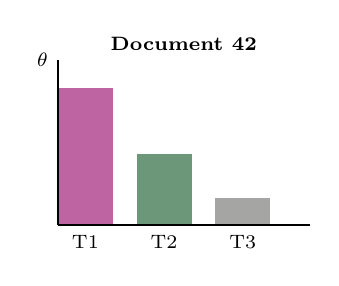
\begin{tikzpicture}[yscale=0.5]
                % Bar chart sketch
                \fill[sgsssMagenta!70] (0,0) rectangle (0.7,3.5);
                \fill[sgsssGreen!70] (1.0,0) rectangle (1.7,1.8);
                \fill[sgsssBlack!40] (2.0,0) rectangle (2.7,0.7);

                % Axis
                \draw[thick] (0,0) -- (3.2,0);
                \draw[thick] (0,0) -- (0,4.2);

                % Labels
                \node[below, font=\scriptsize] at (0.35,0) {T1};
                \node[below, font=\scriptsize] at (1.35,0) {T2};
                \node[below, font=\scriptsize] at (2.35,0) {T3};
                \node[left, font=\scriptsize] at (0,4.2) {\(\theta\)};

                % Title
                \node[above, font=\scriptsize\bfseries] at (1.6,4.2) {Document 42};
            \end{tikzpicture}
            \end{center}

            {\scriptsize Document 42 is mostly about Topic 1, somewhat about Topic 2, and a little about Topic 3.}
        \end{column}
        \begin{column}{0.48\textwidth}
            \textbf{\color{sgsssGreen} (b) Topic \(\to\) Words}\\[0.1cm]
            {\small Each topic has a distribution over words.}

            \vspace{0.2cm}
            \begin{center}
            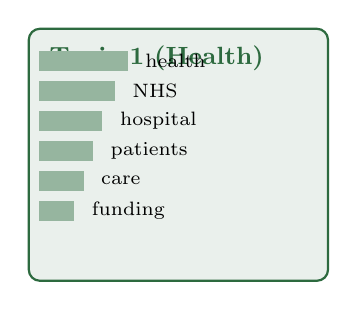
\begin{tikzpicture}
                \tikzset{
                    topicword/.style={font=\scriptsize, anchor=west},
                }
                % Topic box
                \node[rectangle, draw=sgsssGreen, fill=sgsssGreen!10, thick, rounded corners,
                    minimum width=3.8cm, minimum height=3.2cm, anchor=north west] at (0,0) {};
                \node[font=\small\bfseries, anchor=north west, text=sgsssGreen] at (0.15,-0.1) {Topic 1 (Health)};

                % Word list with bars (manually expanded to avoid \foreach in beamer)
                \fill[sgsssGreen!50] (0.15,-0.55) rectangle (1.27,-0.30);
                \node[topicword] at (1.37,-0.425) {health};
                \fill[sgsssGreen!50] (0.15,-0.93) rectangle (1.11,-0.68);
                \node[topicword] at (1.21,-0.805) {NHS};
                \fill[sgsssGreen!50] (0.15,-1.31) rectangle (0.95,-1.06);
                \node[topicword] at (1.05,-1.185) {hospital};
                \fill[sgsssGreen!50] (0.15,-1.69) rectangle (0.83,-1.44);
                \node[topicword] at (0.93,-1.565) {patients};
                \fill[sgsssGreen!50] (0.15,-2.07) rectangle (0.71,-1.82);
                \node[topicword] at (0.81,-1.945) {care};
                \fill[sgsssGreen!50] (0.15,-2.45) rectangle (0.59,-2.20);
                \node[topicword] at (0.69,-2.325) {funding};
            \end{tikzpicture}
            \end{center}

            {\scriptsize The highest-probability words characterise the topic's theme.}
        \end{column}
    \end{columns}
\end{frame}

% -------------------------------------------------------
% Slide 5: Example — topics from parliamentary debates
% -------------------------------------------------------
\begin{frame}{Example: Topics from Parliamentary Debates}
    \small
    {\footnotesize LDA with \(K=4\) topics fitted to UK House of Commons debates. Top 10 words per topic:}

    \vspace{0.2cm}
    \begin{tabular}{@{}cl@{}}
        \toprule
        \textbf{Topic} & \textbf{Top 10 Words} \\
        \midrule
        \textbf{\color{sgsssMagenta} 1 --- Health} & health, NHS, hospital, patients, care, funding, treatment, service, staff, mental \\[0.15cm]
        \textbf{\color{sgsssGreen} 2 --- Education} & education, school, university, students, teachers, learning, skills, children, funding, curriculum \\[0.15cm]
        \textbf{\color{sgsssBlack} 3 --- Economy} & economy, growth, tax, business, employment, trade, investment, inflation, budget, debt \\[0.15cm]
        \textbf{\color{sgsssMagenta!60!sgsssBlack} 4 --- Security} & security, defence, military, police, terrorism, intelligence, border, crime, forces, threat \\
        \bottomrule
    \end{tabular}

    \vspace{0.3cm}
    \begin{exampleblock}{Observation}
        \footnotesize
        The algorithm has no knowledge of politics --- it discovers these groupings purely from \textbf{word co-occurrence patterns}.
        Labels (Health, Education, etc.) are assigned by the researcher after inspection.
    \end{exampleblock}
\end{frame}

% -------------------------------------------------------
% Slide 6: Choosing K (number of topics)
% -------------------------------------------------------
\begin{frame}{Choosing \(K\): The Number of Topics}
    \begin{alertblock}{Why it matters}
        \(K\) is set \textit{by the researcher} before fitting the model. Too few topics conflate distinct themes; too many produce fragmented, uninterpretable topics.
    \end{alertblock}

    \textbf{Approaches to selecting \(K\):}
    \begin{itemize}\setlength\itemsep{0pt}
        \item \faIcon{chart-line} \textbf{Coherence scores} --- automated measure of how semantically related top words are within each topic
        \item \faIcon{chart-bar} \textbf{Held-out likelihood} --- how well the model predicts unseen documents
        \item \faIcon{user-check} \textbf{Human judgement} --- do the topics make substantive sense to domain experts?
    \end{itemize}

    \vspace{0.2cm}
    \begin{exampleblock}{Practical advice}
        \footnotesize
        Try multiple values of \(K\) (e.g., 5, 10, 15, 20). Inspect and compare results. There is \textbf{no single ``correct'' \(K\)} --- the best choice depends on your research question.
    \end{exampleblock}
\end{frame}

% -------------------------------------------------------
% Slide 7: Interpreting and validating topics
% -------------------------------------------------------
\begin{frame}{Interpreting and Validating Topics}
    \small
    \textbf{How to interpret topics:}
    \begin{itemize}\setlength\itemsep{0pt}
        \item \faIcon{list-ol} Read the \textbf{top words} for each topic --- do they form a coherent theme?
        \item \faIcon{file-alt} Examine \textbf{high-loading documents} --- read texts most strongly associated with each topic
        \item \faIcon{tags} Assign \textbf{labels} carefully --- resist the temptation to over-interpret a word list
    \end{itemize}

    \vspace{0.2cm}
    \textbf{External validation:}
    \begin{itemize}\setlength\itemsep{0pt}
        \item Compare topic assignments with \textbf{known metadata} (e.g., committee, policy area)
        \item Check topic prevalence over \textbf{time} --- do trends match known events?
    \end{itemize}

    \vspace{0.2cm}
    \begin{alertblock}{Common pitfalls}
        \footnotesize
        \textbf{Junk topics} (stopwords, boilerplate) \(\cdot\)
        \textbf{Over-splitting} (one theme spread across several topics) \(\cdot\)
        \textbf{Label bias} (reading meaning into vague word lists)
    \end{alertblock}
\end{frame}

% -------------------------------------------------------
% Slide 8: Structural Topic Models (STM)
% -------------------------------------------------------
\begin{frame}{Structural Topic Models (STM)}
    \small
    STM extends LDA by allowing \textbf{document-level metadata} (e.g., party, year, author) to influence topic \textbf{prevalence} and \textbf{content}.

    \vspace{0.1cm}
    \begin{columns}[T]
        \begin{column}{0.52\textwidth}
            \textbf{What STM adds:}
            \begin{itemize}\setlength\itemsep{0pt}
                \item \textbf{Topic prevalence} can vary with covariates\\
                    {\scriptsize e.g., ``Health'' topic more prevalent in Labour speeches}
                \item \textbf{Topic content} (word use) can vary\\
                    {\scriptsize e.g., Labour and Conservative use different words when discussing health}
            \end{itemize}
        \end{column}
        \begin{column}{0.44\textwidth}
            \begin{center}
            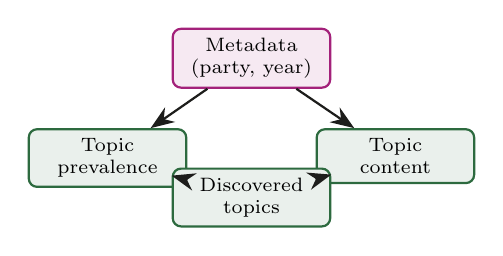
\begin{tikzpicture}[node distance=0.6cm]
                \tikzset{
                    stm node/.style={rectangle, draw=sgsssGreen, fill=sgsssGreen!10, thick,
                        rounded corners=3pt, minimum width=2cm, minimum height=0.6cm, align=center, font=\scriptsize},
                    meta node/.style={rectangle, draw=sgsssMagenta, fill=sgsssMagenta!10, thick,
                        rounded corners=3pt, minimum width=2cm, minimum height=0.6cm, align=center, font=\scriptsize},
                }
                \node[meta node] (meta) {Metadata\\(party, year)};
                \node[stm node, below left=0.5cm and -0.2cm of meta] (prev) {Topic\\prevalence};
                \node[stm node, below right=0.5cm and -0.2cm of meta] (cont) {Topic\\content};
                \node[stm node, below=1.0cm of meta] (topics) {Discovered\\topics};

                \draw[arrow style] (meta) -- (prev);
                \draw[arrow style] (meta) -- (cont);
                \draw[arrow style] (prev) -- (topics);
                \draw[arrow style] (cont) -- (topics);
            \end{tikzpicture}
            \end{center}
        \end{column}
    \end{columns}

    \vspace{0.1cm}
    \begin{exampleblock}{Key reference}
        \footnotesize
        Roberts, Stewart \& Tingley (2014). \textit{``stm: R Package for Structural Topic Models.''}
        See also Roberts et al.\ (2014), \textit{American Journal of Political Science}.
    \end{exampleblock}
\end{frame}

% -------------------------------------------------------
% Slide 9: Strengths and limitations
% -------------------------------------------------------
\begin{frame}{Strengths and Limitations}
    \small
    \begin{columns}[T]
        \begin{column}{0.47\textwidth}
            \textbf{\color{sgsssGreen} Strengths}
            \begin{itemize}\setlength\itemsep{0pt}
                \item \faIcon{expand-arrows-alt} \textbf{Scalable} --- can handle thousands or millions of documents
                \item \faIcon{tag} \textbf{No labelled data required} --- fully unsupervised
                \item \faIcon{search} \textbf{Exploratory power} --- discovers themes the researcher may not have anticipated
                \item \faIcon{project-diagram} \textbf{Mixed membership} --- documents can belong to multiple topics
            \end{itemize}
        \end{column}
        \begin{column}{0.47\textwidth}
            \textbf{\color{sgsssMagenta} Limitations}
            \begin{itemize}\setlength\itemsep{0pt}
                \item \faIcon{random} \textbf{Bag-of-words} --- ignores word order and syntax
                \item \faIcon{sliders-h} \textbf{Sensitive to \(K\)} --- results change with the number of topics
                \item \faIcon{broom} \textbf{Preprocessing matters} --- stopwords, stemming, and rare-word thresholds affect output
                \item \faIcon{dice} \textbf{Not deterministic} --- different random seeds can yield different solutions
            \end{itemize}
        \end{column}
    \end{columns}

    \vspace{0.3cm}
    {\small \faIcon{info-circle} Topic modelling is best used as an \textbf{exploratory} tool. Always validate results with close reading and domain knowledge.}
\end{frame}

% -------------------------------------------------------
% Slide 10: Next up
% -------------------------------------------------------
\begin{frame}{Next Up}
    \begin{center}
        {\Large \alert{Practical 3: Topic Modelling}}\\[0.5cm]
        \begin{itemize}
            \item Preprocess a corpus of parliamentary debates for topic modelling
            \item Fit LDA models with different values of \(K\)
            \item Inspect topic--word distributions and document--topic assignments
            \item Evaluate topic quality using coherence scores
            \item Visualise topics and their prevalence over time
        \end{itemize}
        \vspace{0.5cm}
        {\normalsize Open the \textbf{Practical 3} notebook in Google Colab\\(Python or R --- your choice!)}
    \end{center}
\end{frame}

\end{document}
